The two round strategy works well in our framework, we explore further to look at an advanced adaptive data analysis algorithm - multiple round algorithm.
\begin{example}[Two Round Algorithm]
    \[
    %
        \kw{twoRounds(k)} \triangleq
    \begin{array}{l}
           \clabel{ a \leftarrow []}^{1} ; \\
            \clabel{\assign{j}{k} }^{2} ; \\
            \ewhile ~ \clabel{j > 0}^{3} ~ \edo ~ \\
            \Big(
             \clabel{\assign{x}{\query(\chi[k - j]\cdot \chi[k])} }^{4}  ; \\
             \clabel{\assign{j}{j-1}}^{5} ;\\
            \clabel{a \leftarrow x :: a}^{6}       \Big);\\
            \clabel{l \leftarrow (\mathrm{sign}\big (\sum_{i\in [k]} \chi[i]\times\ln\frac{1+a[i]}{1-a[i]} \big ))}^{7}\\
        \end{array}
    \]
    %
    \begin{algorithm}
    \footnotesize
    \caption{A two-round analyst strategy for random data (The example in  \cite{dwork2015preserving})}
    \label{alg:twoRound}
    \begin{algorithmic}
    \REQUIRE Mechanism $\mathcal{M}$ with a hidden data set $D \in \{-1,+1\}^{n\times (k+1)} \subset \dbdom$.
    \STATE  {\bf for}\ $j\in [k]$\ {\bf do}.  
    \STATE \qquad {\bf define} $q_j(d)=d(j)\cdot d(k)$ where $d \in \{D(i) ~|~ i = 0, \cdots, n\} \subseteq \{-1,+1\}^{k+1}$.
    \STATE \qquad {\bf let} $a_j=\mathcal{M}(q_j)$ 
    \STATE \qquad \COMMENT{In the line above, $\mathcal{M}$ computes approx. the exp. value  of $q_j$ over $D$. So, $a_j\in [-1,+1]$.}
    \STATE {\bf define} $q_{k}(d)= d(k) \cdot \mathrm{sign}\big (\sum_{i\in [k]} x(i) \cdot \ln\frac{1+a_i}{1-a_i} \big )$ where $x\in \{-1,+1\}^{k+1}$.
    \STATE\COMMENT{In the line above,  $\mathrm{sign}(y)=\left \{ \begin{array}{lr} +1 & \mathrm{if}\ y\geq 0\\ -1 &\mathrm{otherwise} \end{array} \right . $.}
    \STATE {\bf let} $a_{k+1}=\mathcal{M}(q_{k+1})$
    \STATE\COMMENT{In the line above,  $\mathcal{M}$ computes approx. the exp. value  of $q_{k+1}$ over $X$. So, $a_{k+1}\in [-1,+1]$.}
    \RETURN $a_{k+1}$.
    \ENSURE $a_{k+1}\in [-1,+1]$
        % \ENSURE 
    \end{algorithmic}
    \end{algorithm}
    %
%
    \end{example}

\begin{example}[Multiple Round Algorithm]
%
\[
%
\kw{multipleRounds(k, c)} \triangleq
\begin{array}{l}
     \left[j \leftarrow k \right]^1 ; \\
    \left[I \leftarrow [] \right]^2; \\
    \ewhile ~ \clabel{j > 0}^{3} ~ \edo ~ \\
    \Big(
    \clabel{\assign{j}{j-1}}^{4} ;\\
    \left[p \leftarrow c \right]^5; \\
    \left[ a \leftarrow \query (\chi[I]) \right]^6;\\
    \left[I \leftarrow \mathrel{\mathsf{update}} ( {I}, (a, p))  \right]^7
    \Big) 
\end{array}
\]
%
\begin{algorithm}
\footnotesize
\caption{A multi-round analyst strategy for random data base \cite{dwork2015preserving}}
\label{alg:multiRound}
\begin{algorithmic}
\REQUIRE Mechanism $\mathcal{M}$ with a hidden state $X\in [N]^{n}$ sampled u.a.r., control set size $c$
\STATE Define control dataset $C = \{0,1, \cdots, c - 1\}$
\STATE Initialize $Nscore(i) = 0$ for $i \in [N]$, $I = \emptyset$ and $Cscore(C(i)) = 0$ for $i \in [c]$
\STATE  {\bf for}\ $j\in [k]$\ {\bf do} 
\STATE \qquad {\bf let} $p=\uniform(0,1)$ 
\STATE \qquad {\bf define} $q (x) = \bernoulli ( p )$ .
\STATE \qquad {\bf define} $qc (x) = \bernoulli ( p )$ .
\STATE \qquad {\bf let} $a = \mathcal{M}(q)$ 
\STATE \qquad {\bf for}\ $i \in [N]$\ {\bf do}
\STATE \qquad \qquad $Nscore(i) = Nscore(i) + (a - p)*(q (i) - p)$ if $i \notin I$
\STATE \qquad {\bf for}\ $i \in [c]$\ {\bf do}
\STATE \qquad \qquad $Cscore(C(i)) = Cscore(C(i)) + (a - p)*(qc (i) - p)$
\STATE \qquad {\bf let} $I = \{i | i\in [N] \land Nscore(i) > \max(Cscore)\}$
\STATE \qquad {\bf let} $D = D \setminus I$ 
\RETURN $D$.
\end{algorithmic}
\end{algorithm}
%
\[
%
\kw{multipleRounds(k, c, N)} \triangleq
\begin{array}{l}
    \clabel{\assign{j}{N}}^0 ; \\
     \clabel{\assign{cs}{0}}^1; \\
     \clabel{\assign{ns}{0}}^2; \\
     \clabel{\assign{I}{0}}^3; \\
     \ewhile ~ \clabel{j > 0}^{4} ~ \edo ~ \\
     \Big(
     \clabel{\assign{j}{j-1}}^{5} ;\\
     \clabel{\assign{cs}{0 + cs}}^6; \\
     \clabel{\assign{ns}{0 + ns}}^7
     \Big); \\
     \clabel{\assign{w}{k}}^{8} ;\\
     \ewhile ~ \clabel{w > 0}^{9} ~ \edo ~ \\
    \Big(
    \clabel{\assign{w}{w-1}}^{10} ;\\
    \left[p \leftarrow c \right]^{11}; \\
    \left[q \leftarrow c \right]^{12}; \\
    \left[ a \leftarrow \query (\chi[I]) \right]^{13};\\
    \clabel{\assign{i}{N}}^{14} ; \\
    \ewhile ~ \clabel{i > 0}^{15} ~ \edo ~ \\
    \Big(
    \clabel{\assign{i}{i-1}}^{16} ;\\
    \clabel{\assign{cs(i)}{cs(i) + (a - p) * (q - p)}}^{17}; \\
    \eif (\clabel{ I < i}^{18}, \clabel{\assign{ns(i)}{{ns(i) + (a - p) * (q - p)}}}^{19},
    \clabel{\assign{ns}{ns(i)}}^{20}    )
    \Big); \\
    \clabel{\assign{i2}{N}}^{21} ; \\
    \ewhile ~ \clabel{i2 > 0}^{22} ~ \edo ~ \\
    \Big(
    \clabel{\assign{i2}{i2-1}}^{23} ;\\
    \eif (\clabel{ns(i2) > \kw{max}(cs)}^{24}, 
    \clabel{\assign{I}{i + I}}^{25},
    \clabel{\assign{I}{I}}^{26})
    \Big)
    \Big) 
\end{array}
\]
weight for Variable: cs of label 6 is: 0 + 1 * N \\
weight for Variable: j of label 5 is: 0 + 1 * N \\
weight for Variable: ns of label 7 is: 0 + 1 * N \\
weight for Variable: csi of label 17 is: 0 + 0 + 1 * k * N \\
weight for Variable: i of label 16 is: 0 + 0 + 1 * k * N \\
weight for Variable: nsi of label 19 is: 0 + 0 + 1 * k * N \\
weight for Variable: nsi of label 20 is: 0 + 0 + 1 * k * N \\
weight for Variable: i2 of label 23 is: 0 + 0 + 1 * k * N \\
weight for Variable: l of label 25 is: 0 + 0 + 1 * k * N \\
weight for Variable: l of label 26 is: 0 + 0 + 1 * k * N \\
weight for Variable: i2 of label 21 is: 0 + 1 * k \\
weight for Variable: i of label 14 is: 0 + 1 * k \\
weight for Variable: a of label 13 is: 0 + 1 * k \\
weight for Variable: q of label 12 is: 0 + 1 * k \\
weight for Variable: p of label 11 is: 0 + 1 * k \\
weight for Variable: w of label 10 is: 0 + 1 * k \\
weight for Variable: w of label 8 is: 1 \\
weight for Variable: ns of label 3 is: 1 \\
weight for Variable: cs of label 2 is: 1 \\
weight for Variable: l of label 1 is: 1 \\
weight for Variable: j of label 0 is: 1 \\
%
\end{example}
  We have seen the two round algorithm above. We show the multiple-round algorithm, which is an advanced algorithm.
 \\
\textbf{Description:}
The multiple round algorithm starts from an initialized empty tracking list $I$, a score called Nscore $ns=0$ , another score Cscore $cs=0$.
There is a hidden database $D$ as well.
% a score called Nscore $ns=0$ , another score Cscore $cs=0$. There is a hidden database $X$ as well.
% It goes $k$ rounds and every round, the two scores $ns$ and $cs$ are updated by a query result. 
% Then the list $I$ is updated by the two scores for every round. After the $r$ rounds, the algorithm returns the columns of the hidden database $X$ not specified in the tracking list $I$, which is $X\setminus I$. 
It goes $k$ rounds and every round, the two scores $ns$ and $cs$ are updated by a query result. 
Then the tracking list is updated by the two scores for every round.  
% Then the list $I$ is updated by the two scores for every round. 
After the $r$ rounds, the algorithm returns the columns of the hidden database $D$ not specified in the tracking list $I$, which is $D \setminus I$. 
\\
The algorithm is written in the while language as $\kw{multipleRounds(k, c)} $ taking two parameters $k$ and $c$ for 
number of iterations and the distribution sampling primitive $c$.
It starts from an initialized empty tracking list $I$ as well,
% a score called Nscore $ns=0$ , another score Cscore $cs=0$. There is a hidden database $X$ as well.
% It goes $k$ rounds and every round, the two scores $ns$ and $cs$ are updated by a query result. 
% Then the list $I$ is updated by the two scores for every round. After the $r$ rounds, the algorithm returns the columns of the hidden database $X$ not specified in the tracking list $I$, which is $X\setminus I$. 
It goes $k$ rounds and every round, construct the query $\query(\chi[I])$
and obtain the query result $a$.
Then, the tracking list $I$ is updated by a query result. 
% Then the list $I$ is updated by the two scores for every round. 
After the $r$ rounds, the algorithm returns the columns of the hidden database $D$ not specified in the tracking list $I$.
The $\mathrel{\mathsf{update}} ( {I}, (a, p))$ function takes $I, a, p$ as input and compute the updated results for $I$.
$\mathsf{update}$ function is used here to simplify the complex update computation of Nscore, Cscore and the tracking list $I$.
It will not change our analysis because these functions provides enough information through their arguments.%

% It uses a loop for the $k$ rounds computation and. We use functions $update\_nscore(p,a)$,$update\_cscore(p,a)$,$update(I,ns,cs)$ to simplify the complex update computation of Nscore, Cscore and the tracking list $I$. It will not change our analysis because these functions provides enough information through their arguments.
% As described in the two round algorithm, the multi-round algorithm has a loop as well.
% compare to two round algorithm
In comparison with the two round algorithm, the query asked in each iteration is not independent  in the multiple round one any more. 
The query in one iteration $j$ now depends on the tracking list $I$ from its previous iteration $j-1$, which is updated by the query result at the same iteration $j-1$. We can easily see the connection between queries from different iterations.
% the result of the query from previous iteration,
% so that the query ask at the $j^{th}$ iteration is
% $q(p, I)$.
%
%
%
\begin{figure}
\begin{center}
%
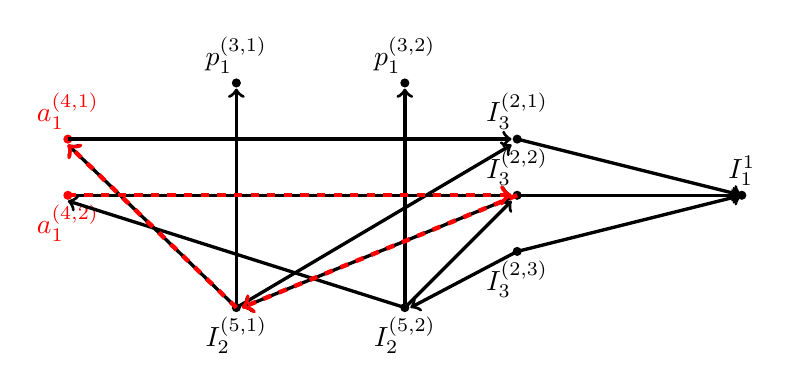
\begin{tikzpicture}[scale=\textwidth/17cm,samples=200]
%%% The nodes represents the k query in the first round
\filldraw[red] (0, 3) circle (2pt) node [anchor=south]{$a_1^{(4,1)}$};
\filldraw[black] (3, 4) circle (2pt) node [anchor=south]{$p_1^{(3,1)}$};
% \filldraw[black] (6, 2) circle (2pt) node [anchor=south]{$q^4_3$};
\filldraw[black] (6, 4) circle (2pt) node [anchor=south]{$p_1^{(3,2)}$};
\filldraw[black] (8, 3) circle (2pt) node [anchor=south]{$I_3^{(2,1)}$};
%%%%%% The nodes represents the n^k queries in the second round
\filldraw[red] (0, 2) circle (2pt) node [anchor=north]{$a_1^{(4,2)}$};
\filldraw[black] (3, 0) circle (2pt) node [anchor=north]{$I_2^{(5,1)}$};
% \filldraw[black] (6, 0) circle (2pt) node [anchor=north]{$q^{3, 7}_{k+1}$};
\filldraw[black] (6, 0) circle (2pt) node [anchor=north]{$I_2^{(5,2)}$};
\filldraw[black] (8, 1) circle (2pt) node [anchor=north]{$I_3^{(2,3)}$};
\filldraw[black] (8, 2) circle (2pt) node [anchor=south]{$I_3^{(2,2)}$};
\filldraw[black] (12, 2) circle (2pt) node [anchor=south]{$I_1^{1}$};
%%%%%The edges between a and I
%%%%% (a1(4,1), I3(2,1))
\draw[very thick, ->] (0, 3)  -- (7.9, 3) ;
%%%%% (a1(4,2), I3(2,2))
\draw[very thick, ->] (0, 2)  -- (7.9, 2) ;
%%%%%% The edges represents their dependency relations GROUP between I3 and I1
\draw[very thick,<-] (12, 2)  -- (8, 2) ;
\draw[very thick,->] (8, 2) -- (3.1, 0) ;
%
\draw[very thick,<-] (12, 2)  -- (8, 1) ;
\draw[very thick,->] (8, 1) -- (6.1, 0) ;
%
\draw[very thick,<-] (12, 2)  -- (8, 3) ;
%
%%%%%% The edges represents their dependency relations GROUP between I2 and others
%%%%%% The edges represents their dependency relations GROUP between I2(5,1) and others
\draw[very thick, ->] (3, 0)  -- (0, 2.9) ;
\draw[very thick, ->] (3, 0)  -- (3, 3.9) ;
\draw[very thick, ->] (3, 0)  -- (7.9, 2.9) ;
%%%%%% The edges represents their dependency relations GROUP between I2(5,2) and others
\draw[very thick, ->] (6, 0)  -- (0, 1.9) ;
\draw[very thick, ->] (6, 0)  -- (6, 3.9) ;
\draw[very thick, ->] (6, 0)  -- (7.9, 1.9) ;
%%%% The longest path representing the adaptivity
\draw[ultra thick, red, ->, dashed] (0, 2) -- (7.9, 2);
\draw[ultra thick, red, ->, dashed] (8, 2) -- (3.1, 0);
\draw[ultra thick, red, ->, dashed] (3, 0)  -- (0, 2.9);
\end{tikzpicture}
\end{center}
    \caption{the variable dependency graph for multi round algorithm}
    \label{fig:multi-round-graph-ssa}
\end{figure}
%
The adaptivity is 1 computed from the graph.
The query-based dependency graph is a subgraph of the variable dependency graph for multi round algorithm.



\begin{example}[Sequence with Single Variable Linear Data Value Dependency]
    %
    %
    \[
    %
        \kw{seq()} \triangleq 
    \begin{array}{l} 
           \clabel{ \assign{x}{\chi[0]}}^{0} ; \\
            \clabel{\assign{y}{\chi[x + 1]} }^{1} ; \\
            \clabel{\assign{z}{\chi[y + 1]}}^{2}; \\
             \clabel{\assign{w}{\chi[z + 1]} }^{3}
        \end{array}
    \]
    Analysis Result: $ \progA( \kw{seq()}) = 4$
    \end{example}
%
\begin{example}[Sequence with Multiple Variables Data Value Dependency]
    %
    %
    \[
    %
        \kw{seqMultiVar()} \triangleq 
    \begin{array}{l} 
           \clabel{ \assign{x}{\chi[0]}}^{0} ; \\
            \clabel{\assign{y}{\chi[x + 1]} }^{1} ; \\
            \clabel{\assign{z}{\chi[y + x]}}^{2}; \\
             \clabel{\assign{w}{\chi[z + 1] \cdot \chi[y]} }^{3}
        \end{array}
    \]
    Analysis Result: $ \progA(\kw{seqMultiVar()}) = 4$
\end{example}
%
    \begin{example}[If with Data-Value Dependency Separated]
        %
        %
        \[
        %
        \kw{ifValueDependency}(k) \triangleq 
        \begin{array}{l}
           \quad \clabel{ \assign{z}{\query(\chi[0])}}^{0} ; \\
           \quad \clabel{\assign{x}{k / 2} }^{1} ; \\
           \quad \eif(\clabel{x < 0}^2, \\
           \quad \clabel{\assign{y}{\query(\chi[z])}}^{3}, \\ 
           \quad \clabel{\assign{y}{\query(\chi[0])}}^{4})
            \end{array}
        \]
        Analysis Result: $ \progA( \kw{ifControlDependency()}) = 3$
    \end{example}

        \begin{example}[If with Data-Control Dependency Overlapped]
            %
            %
            \[
            %
            \kw{ifControlDependency()} \triangleq 
            \begin{array}{l}
                \clabel{ \assign{z}{\query(\chi[0])}}^{0} ; \\
                \clabel{\assign{x}{\query(\chi[z])} }^{1} ; \\
                \eif(\clabel{x < 0}^{2}, 
                \clabel{\assign{y}{\query(\chi[0] + \chi[1])}}^{3}, 
                \clabel{\assign{y}\query{(\chi[0])}}^{4})
            \end{array}
            \]
            %
            Analysis Result: $ \progA( \kw{ifControlDependency()}) = 3$
            \end{example}


            \begin{example}[Simple While with Recursive Data-Value Dependency]
                %
                %
                \[
                %
                \kw{whileRec}() \triangleq
                \begin{array}{l}
                    \clabel{ \assign{j}{10000} }^{0} ; \\
                    \clabel{ \assign{a}{\query(\chi[0])} }^{1} ; \\
                        \ewhile ~ \clabel{j > 0}^{2} ~ \edo ~ \\
                        \Big(
        \clabel{\assign{x}{\query(\chi[a]) }}^{3}  ; \\
        \clabel{\assign{a}{x + a}}^{4} ;\\
                        \clabel{\assign{j}{j-1}}^{5}       \Big)
                    \end{array}
                \]
                Analysis Results: $ \progA(\kw{whileRec}(k)) = 1 + k$
            \end{example}
%
        \begin{example}[Simple While with Multi-Path Data-Value Dependency]
        %
        %
        \[
        %
        \kw{whileMultiplePath(k)} \triangleq 
        \begin{array}{l}
            \clabel{ \assign{j}{k}}^{0} ; \\
            \clabel{ \assign{x}{\query(\chi[0])} }^{1} ; \\
                \ewhile ~ \clabel{j > 0}^{2} ~ \edo ~ \\
                \Big(
                 \clabel{\assign{j}{j-1}}^{3} ;\\
                 \eif(\clabel{j \% 2 == 0}^{4}, 
                 \clabel{\assign{y}{\chi[x]}}^{5}, 
                 \clabel{\assign{w}{\chi[x]}}^{6});\\           
                 \clabel{\assign{x}{\query(\chi(\ln(y)))} }^{7} \Big)
            \end{array}
        \]
        Analysis Results: $ \progA(\kw{whileMultiplePath}(k)) = 1 + 2 * k $ --> Over-Approximated
    \end{example}
%
        \begin{example}[Simple While with Recursive Multiple-Variable Data-Value Dependency]
            \[
            %
            \kw{whileMultipleVar}(k) \triangleq 
            \begin{array}{l}
            \clabel{\assign{j}{k} }^{0} ; \\
            \clabel{ \assign{x}{\query(\chi[0])}}^{1} ; \\
                \clabel{ \assign{y}{\query(\chi[1])}}^{2} ; \\
                    \ewhile ~ \clabel{j > 0}^{3} ~ \edo ~ \\
                    \Big(
                     \clabel{\assign{j}{j-1}}^{4} ;\\
                     \clabel{\assign{z}{\query(\chi(x + \ln(y)))} }^{5}  ; \\
                     \clabel{ \assign{x}{\query(\chi[z])}}^{6} ; \\
                     \clabel{ \assign{y}{\query(\chi[z])}}^{7} 
                    \Big)
                \end{array}
            \]
            Analysis Results: $ \progA(\kw{whileMultipleVar}(k)) = 1 + 2 * k $
        \end{example}
            %
            %
            \begin{example}[Simple While with Data-Value and Data-Control Dependency]
                %
                \[
                \kw{whileValueControlDependency}() \triangleq
                \begin{array}{l}
                    \clabel{ \assign{x}{\query(\chi[0])} }^{0} ; \\
                    \clabel{ \assign{z}{\query(\chi[0])} }^{1} ; \\
                        \ewhile ~ \clabel{x > 0}^{2} ~ \edo ~ \\
                        \Big(
                        \clabel{\assign{x}{\query(\chi(z))} }^{3}  ; \\
                        \clabel{\assign{z}{\query(\chi(x))}}^{4}
                      \Big)
                    \end{array}
                \]
                Analysis Results: $ \progA(\kw{whileValueControlDependency}(k)) = 1 + 2 * k $
            \end{example}
%
            \begin{example}[Simple While with MultiplePath Data-Value and Data-Control Dependency]
                %
                \[
                    %
                    \begin{array}{l}
                    \kw{whileMultiplePathValueControlDependency}(k) \triangleq\\
                        \clabel{ \assign{x}{\query(k)}}^{0} ; \\
                        \clabel{\assign{y}{0} }^{1} ; \\
           \ewhile ~ \clabel{x > 0}^{2} ~ \edo ~ \\
           \Big(
            \eif(\clabel{y > 0}^{3}, 
            \clabel{\assign{y}{\query(\chi[12])}}^{4}, 
            \clabel{\assign{w}{\query(\chi[9])}}^{5});           
            \\
            \clabel{\assign{x}{x-1}}^{6}\Big);\\
            \clabel{\assign{y}{\query(\chi(\ln(y)))} }^{7} 
                        \end{array}
                    \]
                    Analysis Results: $ \progA(\kw{whileMultiplePathValueControlDependency}(k)) = 2 + k $
                \end{example}
               %
                \begin{example}[Nested While with Recursive Data-Value Dependency]
                    %
                    %
                    \[
                    %
                    \kw{nestWhileValueDependency}(k) \triangleq 
                    \begin{array}{l}
                        \clabel{ \assign{i}{k} }^{0} ; \\
                        \clabel{\assign{x}{\query(\chi[0])}}^{1} ; \\
           \ewhile ~ \clabel{i > 0}^{2} ~ \edo ~ \\
           \Big(
            \clabel{\assign{i}{i-1}}^{3} ;\\
            \clabel{\assign{j}{k}}^{4} ;\\
            \clabel{\assign{y}{\query(\chi(\ln(x)))} }^{5}  ; \\
            \ewhile ~ \clabel{j > 0}^{6} ~ \edo ~ \\
            \Big(
             \clabel{\assign{j}{j-1}}^{7};\\
             \clabel{\assign{x}{\query(\chi(\ln(x)))} }^{8}
             \Big) \Big)
                        \end{array}
                    \]
                    Analysis Results: $ \progA(\kw{nestWhileValueDependency}(k)) = 2 + k^2 $
                \end{example}

                    \begin{example}[Nested While with Nested Recursive Data-Value Dependency Across Outer and Inner Loop]
                        %
                        %
                        \[
                        %
           \kw{nestedWhileRecAcross}(k) \triangleq 
                        \begin{array}{l}
           \clabel{ \assign{i}{k} }^{0} ; \\
           \clabel{\assign{x}{\query(\chi[0])}}^{1} ; \\
               \ewhile ~ \clabel{i > 0}^{2} ~ \edo ~ \\
               \Big(
                \clabel{\assign{i}{i-1}}^{3} ;\\
                \clabel{\assign{j}{k}}^{4} ;\\
                \ewhile ~ \clabel{j > 0}^{5} ~ \edo ~ \\
                \Big(
                 \clabel{\assign{j}{j-1}}^{6};\\
                 \clabel{\assign{y}{\query(\chi(x) + \chi(1))} }^{7}
                 \Big); \\
                \clabel{\assign{x}{\query(\chi(\ln(y)))} }^{8}
                 \Big)
           \end{array}
                        \]
                        Analysis Results: $ \progA(\kw{nestedWhileRecAcross}(k)) = 1 + 2 * k $
                    \end{example}
                %
            
                        \begin{example}[Nested While with Nested Recursive Multiple Variable 
           Data-Value Dependency Across Outer and Inner Loop]
           %
           \[
           %
           \kw{nestedWhileMultiVarRecAcross}(k) \triangleq 
           \begin{array}{l}
               \clabel{\assign{i}{k} }^{0} ; \\
               \clabel{ \assign{x}{\query(\chi[0])}}^{1} ; \\
               \clabel{ \assign{y}{\query(\chi[1])}}^{2} ; \\
          \ewhile ~ \clabel{i > 0}^{3} ~ \edo ~ \\
          \Big(
           \clabel{\assign{i}{i-1}}^{4} ;\\
           \clabel{\assign{j}{k}}^{5} ;\\
           \clabel{\assign{y}{\query(\chi(\ln(x) + y))} }^{6}  ; \\
           \ewhile ~ \clabel{j > 0}^{7} ~ \edo ~ \\
           \Big(
            \clabel{\assign{j}{j-1}}^{8};\\
            \clabel{\assign{x}{\query(\chi(\ln(y))+\chi[x])} }^{9}
            \Big) \Big)
               \end{array}
           \]
           Analysis Results: $ \progA(\kw{nestedWhileMultiVarRecAcross}(k)) = 1 + k + k^2$
           \\
           weight for Variable: j of label 6 is: 0 + 0 + 1 * k * k\\
           weight for Variable: y of label 7 is: 0 + 0 + 1 * k * k\\
           weight for Variable: j of label 4 is: 0 + 1 * k\\
           weight for Variable: i of label 3 is: 0 + 1 * k\\
           weight for Variable: x of label 8 is: 0 + 1 * k\\
           weight for Variable: x of label 1 is: 1\\
           weight for Variable: i of label 0 is: 1\\
           \end{example}
                    
           \begin{example}[Nested While with MultiplePath and Nested Recursive Multiple Variable 
               Data-Value Dependency Across Outer and Inner Loop]
               %
               We then show a more complex example with nested while command and nested data-flow across the outer and inner while loop through multiple variables.
               This example also contains the if command with data dependency occurred through the if guard.
               %
               \[
               %
               \begin{array}{l}
               \kw{nestedWhileMultiPathMultiVarRecAcross}(k) \triangleq \\
          \clabel{\assign{i}{k} }^{0} ; \\
          \clabel{ \assign{x}{\query(\chi[0])}}^{1} ; \\
          \clabel{ \assign{y}{\query(\chi[1])}}^{2} ; \\
              \ewhile ~ \clabel{i > 0}^{3} ~ \edo ~ \\
              \Big(
               \clabel{\assign{i}{i-1}}^{4} ;\\
               \clabel{\assign{j}{k}}^{5} ;\\
               \eif(\clabel{x > 0}^6, \clabel{\assign{y}{\query(\chi(\ln(x) + y))} }^{7},
               \clabel{\assign{y}{\query(\chi(x))} }^{8} )
                ; \\
               \ewhile ~ \clabel{j > 0}^{9} ~ \edo ~ \\
               \Big(
                \clabel{\assign{j}{j-1}}^{10};\\
                \clabel{\assign{x}{\query(\chi(\ln(y))+\chi[x])} }^{11}
                \Big) \Big)
          \end{array}
               \]
               Analysis Results: $ \progA(\kw{nestedWhileMultiPathMultiVarRecAcross}(k)) = 1 + k + k^2$
               \\
               weight for Variable: j of label 10 is: 0 + 0 + 1 * k * k \\
               weight for Variable: x of label 11 is: 0 + 0 + 1 * k * k \\
               weight for Variable: y of label 7 is: 0 + 1 * k \\
               weight for Variable: y of label 8 is: 0 + 1 * k \\
               weight for Variable: j of label 5 is: 0 + 1 * k \\
               weight for Variable: i of label 4 is: 0 + 1 * k \\
               weight for Variable: y of label 2 is: 1 \\
               weight for Variable: x of label 1 is: 1 \\
               weight for Variable: i of label 0 is: 1 \\
               \end{example}

               \begin{example}[Gradient Decent Algorithm]
          \[
          %
          \kw{gradientDecent(step, rate, t, n)} \triangleq
          \begin{array}{l}
                 \clabel{ a \leftarrow []}^{0} ; \\
                  \clabel{\assign{j}{step} }^{1} ; \\
                %   \clabel{\assign{d}{10000000} }^{2} ; \\
                  \ewhile ~ \clabel{j > 0 \land d < t}^{3} ~ \edo ~ \\
                  \Big(
                      \clabel{\assign{d}{\query(2 * (\chi[1] - (\chi[0]\times x )) * (-\chi[0]))} }^{4}  ; \\
                      \clabel{\assign{x}{x - rate * d} }^{4}  ; \\
                   \clabel{\assign{j}{j-1}}^{5} ;\\
                  \clabel{a \leftarrow x :: a}^{6} 
                  \Big);
              \end{array}
          \]
          %
          %
               %
          \end{example}

               \begin{example}[Two Round Odd Elements ]
          We present a variant of the previous two round example in Figure~\ref{fig:tworound_odd}. In this odd example, only the data at odd index of the database is used.
          %
          {\small
          \begin{figure}
          \begin{subfigure}{.4\textwidth}
          \begin{centering}
          $\begin{array}{l}
              % \left[j \leftarrow 0 \right]^1 ; \\
             \clabel{ \assign{a}{0}  }^{1} ; \\
              \clabel{\assign{j}{0} }^{2} ; \\
              \eloop ~ \clabel{3}^{3} ~ \edo ~ \\
             \quad 
               \eif ( \clabel{( j \% 2 == 0)}^{4}\\
               \quad \quad ,\clabel{ \assign{x}{ q(\chi[j+1])} }^{5}  \\
               \quad \quad ,\clabel{\assign{x}{ q(\chi[j]) }}^{6} ) ;\\
               \quad \clabel{\assign{a}{ a+x} }^{7}  ;\\
               \quad \clabel{ \assign{j}{j+1} }^{8}      ;\\
           \clabel{l \leftarrow q(a*\chi[3]) }^{9}\\
          \end{array} $
          \caption{}
          \end{centering}
          \end{subfigure}
          \begin{subfigure}{0.5\textwidth}
          \begin{centering}
          $
          \begin{array}{l}
              \clabel{ \assign{a_1}{0}  }^{1} ; \\
              \clabel{\assign{j_1}{0} }^{2} ; \\
              \eloop ~ \clabel{3}^{3} , 0,  ~ \edo ~ [(j_3, j_1,j_2), (a_3, a_1,a_2)], \\
            \quad 
               \eif ( \clabel{( j_3 \% 2 == 0)}^{4}, [x_3,x_1,x_2], [],[]\\
               \quad \quad ,\clabel{ \assign{x_1}{ q(\chi[j_3+1])} }^{5}  \\
               \quad \quad ,\clabel{\assign{x_2}{ q(\chi[j_3]) }}^{6} ) ;\\
               \quad \clabel{\assign{a_2}{ a_3+x_3} }^{7}  ;\\
               \quad \clabel{ \assign{j_2}{j_3+1} }^{8}      ;\\
           \clabel{l_1 \leftarrow q(a_3*\chi[3]) }^{9}\\
          \end{array}$
          \caption{}
          \end{centering}
          \end{subfigure}
              \vspace{-0.2cm}
              \caption{(a) The two round odd algorithm in labeled {\tt Loop} language, (b) The SSA program for the same example. }
              \label{fig:tworound_odd}
              \vspace{-0.5cm}
          \end{figure}
          }
          \end{example}
          %
          This algorithm only touches the odd part of the database, by adding an extra if statement to checking the index $j$ in Figure~\ref{fig:tworound_odd}(a). The extra complexity is added to handle the newly generated variables in the loop and if statement in the SSA version in Figure~\ref{fig:tworound_odd}(b). 
          The query-based dependency graph does not change a lot compared to the previous two rounds example in Figure~\ref{fig:simpl-two-round-graph}(c), but the node does change according to the trace. We assume $a = n$ in the final memory is the result of the sum of previous query results in the loop.
          We give the trace $t = [q(\chi[1])^{5,[3:1]}, q(\chi[1])^{6,[3:2]}, q(\chi[3])^{5,[3:3]}, q(n* \chi[3])^{9,\emptyset} ]$ and use $q_1$ for $q(\chi[1])$, $q_3$ representing for $q(\chi[3])$, $q_4$ for $q(n* \chi[3])$. The query-based dependency graph based on this trace is shown in Figure~\ref{fig:odd_graphs}(a). We show the red path, which is a sequence of adaptively chosen queries of length $2$. So among the total $4$ queries, we have 2-round adaptive queries. According to the Theorem\ref{thm:gaussiannoise} and \ref{thm:gaussiannoise2}, we will have a tighter upper bound on the generalization error if we know the adaptivity $2$, obtained from the red path in Figure~\ref{fig:odd_graphs}(a). 
          
          Our algorithm {\THESYSTEM} gives us the upper bound on the aforementioned adaptivity $2$. We construct the variable-based weighted dependency graph in Figure~\ref{fig:odd_graphs}(b). The weighted nodes are in the red dashed circle and the red dashed paths show the most weighted path in the graph, with the weight $2$. So, for this two rounds odd algorithm, our system gives a tight upper bound $2$, which can be used to get a better generalization error bound.
          
          
          
          
          \begin{figure}
              \begin{subfigure}{0.4\textwidth}
              \begin{centering}
              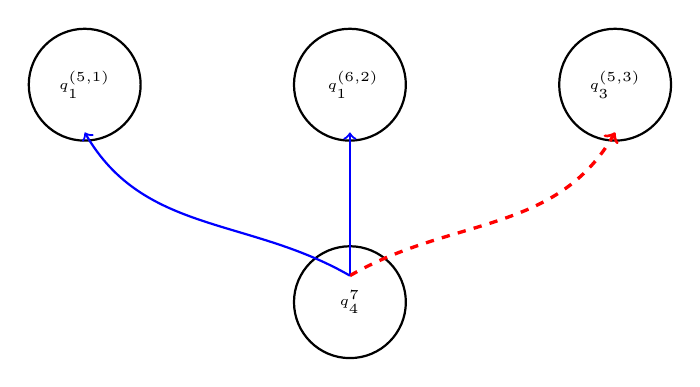
\begin{tikzpicture}[scale=\textwidth/18cm,samples=200]
          %%% The nodes represents the k query in the first round
          % \draw[very thick] (-1,6)  -- (13,6) -- (13,3) -- (-1,3) -- (-1,6);
          % \draw[black] (-2.5, 4) circle (0pt) node [anchor=south]{\textbf{line 4:}};
          \draw[thick] (1, 4.1) circle (30pt) node
          % node[label={above: \small{iteration 1:}}] 
          {\tiny{$q_1^{(5,1)}$}} ;
          \draw[thick] (6, 4.1) circle (30pt) node
          {\tiny{ $q_1^{(6,2)}$}};
           \draw[thick] (11, 4.1) circle (30pt) node 
          {\tiny{$q_3^{(5,3)}$}};
          % \filldraw[black] (-2.5, 0) circle (0pt) node [anchor=south]{\textbf{line 7:}};
          \draw[thick] (6, 0) circle (30pt) node {\tiny{$q_4^7$}};
          \draw[ thick,->, blue] (6, 0.5)  -- (6, 3.2) ;
          \draw[very thick,->, red, dashed] (6, 0.5)  to [out=30,in=240] (11, 3.2) ;
          \draw[ thick,->, blue] (6, 0.5)  to [out=150,in=300]  (1, 3.2) ;
          \end{tikzpicture}
          \caption{}
              \end{centering}
              \end{subfigure}
              \begin{subfigure}{0.5\textwidth}
              \begin{centering}
              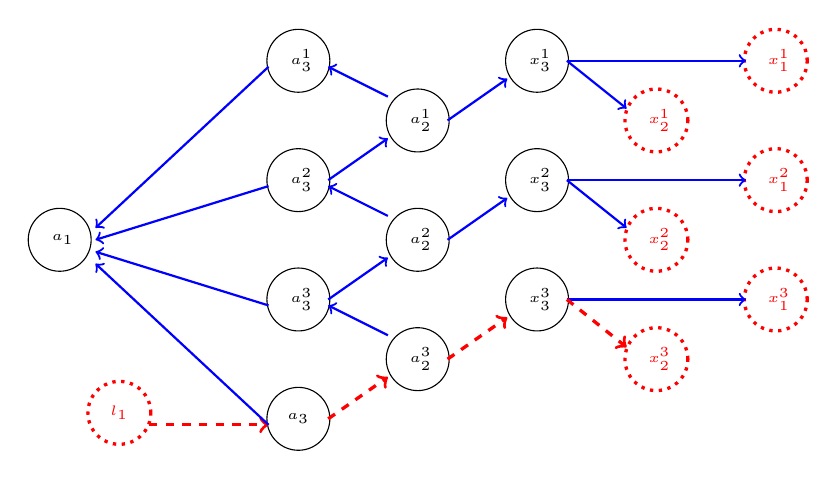
\begin{tikzpicture}[scale=\textwidth/16cm,samples=200]
          %%% The nodes represents the k query in the first round
          % \draw[very thick] (-1,6)  -- (13,6) -- (13,3) -- (-1,3) -- (-1,6);
          % \draw[black] (-2.5, 4) circle (0pt) node [anchor=south]{\textbf{line 4:}};
          % \draw[thick] (1, 1.1) circle (25pt) node
          % % node[label={above: \small{iteration 1:}}] 
          % {\tiny{$q_1^{(5,1)}$}} ;
          \draw[] (2, 5.1) circle (15pt) node
          {\tiny{ $a_1$}};
          \draw[] (6, 8.1) circle (15pt) node
          {\tiny{ $a_3^{1}$}};
          \draw[very thick, red, dotted] (14, 8.1) circle (15pt) node
          {\tiny{ $x_{1}^{1}$}};
          \draw[very thick, red, dotted] (12, 7.1) circle (15pt) node
          {\tiny{ $x_{2}^{1}$}};
          \draw[] (10, 8.1) circle (15pt) node
          {\tiny{ $x_{3}^{1}$}};
          \draw[] (8, 7.1) circle (15pt) node
          {\tiny{ $a_{2}^{1}$}};
          \draw[] (6, 6.1) circle (15pt) node
          {\tiny{ $a_3^{2}$}};
          \draw[very thick, red, dotted] (14, 6.1) circle (15pt) node
          {\tiny{ $x_{1}^{2}$}};
          \draw[very thick, red, dotted] (12, 5.1) circle (15pt) node
          {\tiny{ $x_{2}^{2}$}};
          \draw[] (10, 6.1) circle (15pt) node
          {\tiny{ $x_{3}^{2}$}};
          \draw[] (8, 5.1) circle (15pt) node
          {\tiny{ $a_{2}^{2}$}};
          \draw[very thick, red, dotted] (14, 4.1) circle (15pt) node
          {\tiny{ $x_1^{3}$}};
          \draw[] (6, 4.1) circle (15pt) node
          {\tiny{ $a_3^{3}$}};
          \draw[] (10, 4.1) circle (15pt) node
          {\tiny{ $x_3^{3}$}};
          \draw[very thick, red, dotted] (12, 3.1) circle (15pt) node
          {\tiny{ $x_2^{3}$}};
          \draw[] (8, 3.1) circle (15pt) node
          {\tiny{ $a_{2}^{3}$}};
           \draw[] (6, 2.1) circle (15pt) node 
          {\tiny{$a_3$}};
          % \filldraw[black] (-2.5, 0) circle (0pt) node [anchor=south]{\textbf{line 7:}};
          \draw[very thick, red, dotted] (3, 2.2) circle (15pt) node {\tiny{$l_1$}};
           \draw[very thick,->, red, dashed] (3.5, 2)  -- (5.5, 2) ;
           \draw[very thick,->, red, dashed] (6.5, 2.1)  -- (7.5, 2.8) ;
           \draw[very thick,->, red, dashed] (8.5, 3.1)  -- (9.5, 3.8) ;
           \draw[thick,->, blue] (10.5, 4.1)  -- (13.5, 4.1) ;
            \draw[very thick,->, red, dashed] (10.5, 4.1)  -- (11.5, 3.3) ;
             \draw[thick,->, blue] (7.5, 3.5)  -- (6.5, 4.0) ;
             \draw[thick,->, blue] (6.5, 4.1)  -- (7.5, 4.8) ;
              \draw[thick,->, blue] (8.5, 5.1)  -- (9.5, 5.8) ;
               \draw[thick,->, blue] (10.5, 6.1)  -- (11.5, 5.3) ;
          \draw[thick,->, blue] (10.5, 6.1)  -- (13.5, 6.1) ;
          \draw[thick,->, blue] (7.5, 5.5)  -- (6.5, 6.0) ;
          \draw[thick,->, blue] (6.5, 6.1)  -- (7.5, 6.8) ;
          \draw[thick,->, blue] (8.5, 7.1)  -- (9.5, 7.8) ;
          \draw[thick,->, blue] (10.5, 8.1)  -- (11.5 , 7.3) ;
          \draw[thick,->, blue] (10.5, 8.1)  -- (13.5 , 8.1) ;
          % \draw[thick,->, blue] (8.5, 9.1)  -- (9.5 , 9.8) ;
          % \draw[thick,->, blue] (8, 9.6)  -- (8, 10.6) ;
          \draw[thick,->, blue] (7.5, 7.5)  -- (6.5, 8.0) ;
          \draw[thick,->, blue] (5.5, 8.0)  -- (2.6, 5.3) ;
          \draw[thick,->, blue] (5.5, 6.0)  -- (2.6, 5.1) ;
          \draw[thick,->, blue] (5.5, 4.0)  -- (2.6, 4.9) ;
          \draw[thick,->, blue] (5.5, 2.0)  -- (2.6, 4.7) ;
          % \draw[very thick,->, red] (6, 0.5)  to [out=30,in=240] (11, 3.2) ;
          % \draw[very thick,->, blue] (6, 0.5)  to [out=150,in=300]  (1, 3.2) ;
          \end{tikzpicture}
              \caption{}
              \end{centering}
              \end{subfigure}
              \vspace{-0.3cm}
              \caption{(a) The query-based dependency graph for odd example (b) The SSA variable-based weighted dependency graph for the same example, the node in red dashed circle is weighted.}
              \label{fig:odd_graphs}
              \vspace{-0.3cm}
          \end{figure}